\subsection{Zero field transition}

\subsubsection*{Energy Levels Near Zero Field}
 
In the weak-field (Zeeman) limit, the energy of the $m$-th magnetic sublevel is given
by Eq.~(\ref{eq:W_hyperfine}) :
\begin{equation}
    W_M = g_F\,\mu_0\,B\,M, \qquad M = -F,\,-F+1,\,\ldots,\,+F
    \label{eq:ZF_energy}
\end{equation}
The spacing between adjacent sublevels is:
\begin{equation}
    \Delta W = W_{M+1} - W_M = g_F\,\mu_0\,B
    \label{eq:ZF_spacing}
\end{equation}
which vanishes as $B \to 0$. At exactly zero field all $2F+1$ sublevels become
\textbf{degenerate}, so the distinct quantization axis required for optical pumping
disappears.
 
\subsubsection*{Condition for Optical Pumping}
 
Optical pumping builds a population imbalance by driving $\Delta M = +1$ transitions.
The pumping rate into sublevel $M$ from sublevel $M-1$ is proportional to the transition
probability, which depends on the energy separation $\Delta W$. Defining a dimensionless
pumping parameter :
\begin{equation}
    \eta \equiv \frac{g_F\,\mu_0\,B}{\Gamma_{\text{rel}}}
    \label{eq:pumping_param}
\end{equation}
where $\Gamma_{\text{rel}}$ is the collisional relaxation rate, the steady-state population
imbalance scales as :
\begin{equation}
    \delta p \equiv p_{M_{\max}} - p_{\text{eq}}
    \;\propto\; \frac{\eta^2}{1 + \eta^2}
    \label{eq:pop_imbalance}
\end{equation}
As $B \to 0$, we have $\eta \to 0$ and therefore $\delta p \to 0$ : \textbf{optical pumping
ceases} and the population returns to the thermal equilibrium distribution.
 
\subsubsection*{Transmitted Light Intensity}
 
The transmitted light intensity through the absorption cell follows
Beer-Lambert's law (Eq.~(\ref{eq:beer_lambert})) :
\begin{equation}
    I = I_0\,\exp\!\left(-\sigma_0\,\rho\,\ell\right)
    \label{eq:ZF_BL}
\end{equation}
The effective absorption cross-section $\sigma_0$ depends on the fraction of atoms
available to absorb the 795~nm photons, i.e.\ on the population of sublevels $M < +2$.
In the pumped steady state, most atoms reside in $M = +2$ and cannot absorb; hence
$\sigma_{\text{eff}} \ll \sigma_0$ and $I$ is large. At $B = 0$ the levels are degenerate,
the population is equally distributed, and the absorption reverts to the unpumped value :
\begin{equation}
    \sigma_{\text{eff}}\big|_{B=0} = \sigma_0
    \;\Longrightarrow\;
    I\big|_{B=0} = I_0\,e^{-\sigma_0\,\rho\,\ell} < I_{\text{pumped}}
    \label{eq:ZF_absorption}
\end{equation}
A \textbf{dip} in the transmitted intensity is therefore observed whenever the total
magnetic field at the cell passes through zero (Figure~\ref{fig:ZF_signal}).
 
\begin{figure}[h]
    \centering
    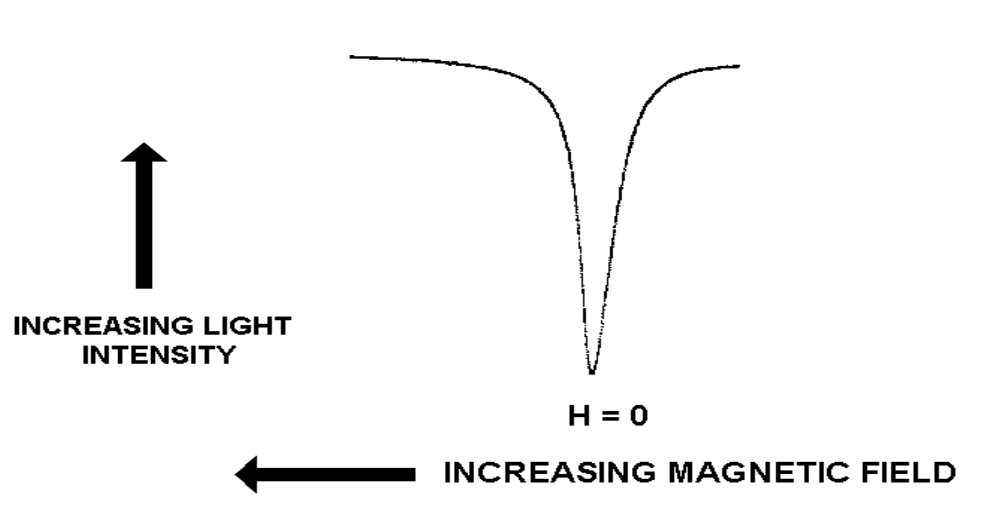
\includegraphics[width=0.55\textwidth]{figures/4e.png}
    \caption{Transmitted light intensity as a function of applied magnetic field.
             A dip is observed at $B = 0$ where all $M$ sublevels are degenerate.}
    \label{fig:ZF_signal}
\end{figure}
 
\subsubsection*{Linewidth of the Zero-Field Signal}
 
The half-width at half-maximum (HWHM) of the zero-field dip can be estimated by
requiring that the Zeeman splitting equal the relaxation-broadened linewidth
$\Gamma_{\text{rel}}$ :
\begin{equation}
    g_F\,\mu_0\,B_{1/2} = \Gamma_{\text{rel}}
    \;\Longrightarrow\;
    B_{1/2} = \frac{\Gamma_{\text{rel}}}{g_F\,\mu_0}
    \label{eq:ZF_linewidth}
\end{equation}
Minimizing $B_{1/2}$ experimentally — by adjusting the compensating coils and the
orientation of the apparatus — drives the residual field at the cell toward zero. The
zero-field signal thus provides a sensitive \textit{in situ} determination of the total
magnetic field, and the minimum achievable linewidth is limited by AC magnetic field
noise at the power-line frequency (50/60~Hz).
 
\subsubsection*{Sweep-Rate Condition}
 
If the magnetic field is swept at a rate $\dot{B}$, the system can follow the equilibrium
population distribution only if the sweep is slow compared to the pumping time
$\tau_p \sim 1/b$ (where $b$ is the optical pumping rate per atom). The adiabaticity
condition is :
\begin{equation}
    \dot{B} \ll \frac{B_{1/2}}{\tau_p}
              = \frac{\Gamma_{\text{rel}}\,b}{g_F\,\mu_0}
    \label{eq:ZF_adiabatic}
\end{equation}
Violating this condition produces time-dependent (transient) effects that are discussed in the Transient Effects section.